\documentclass[Lau,binding=0.6cm,noexaminfo,oneside]{sapthesis}

\usepackage{microtype}
\usepackage[italian]{babel}
\usepackage[utf8]{inputenc}
\usepackage{listings}

%\usepackage{hyperref}
%\hypersetup{pdftitle={Semantic Search App},pdfauthor={Matteo Mancanelli}}

\title{Semantic Search App: strutturazione, correlazione e ricerca semantica dell'informazione multimediale}
\author{Matteo Mancanelli}
\IDnumber{1711823}
\course{Ingegneria Informatica e Automatica}
\courseorganizer{Facoltà di Ingegneria dell'Informazione, Informatica e Statistica}
\AcademicYear{2017/2018}
\copyyear{2018}
\advisor{Prof. Riccardo Rosati}
\authoremail{mancanelli.1711823@studenti.uniroma1.it}

%%%% tikz-er2
\NeedsTeXFormat{LaTeX2e}
\ProvidesPackage{tikz-er2}[2009/01/31 Entity-relationship diagrams using the Tikz library]

\RequirePackage{tikz}
\RequirePackage[normalem]{ulem}  % for the dashed underline

\usetikzlibrary{shapes.geometric}
\usetikzlibrary{arrows}
\usetikzlibrary{matrix}
\usetikzlibrary{chains}
\usetikzlibrary{fit}
\usetikzlibrary{positioning}
\usetikzlibrary{decorations.pathreplacing}
\usetikzlibrary{shadows}
\usetikzlibrary{automata}

\tikzstyle{every entity} = [top color=white, bottom color=blue!30, draw=blue!50!black!100]
\tikzstyle{every weak entity} = [drop shadow={shadow xshift=.7ex, shadow yshift=-.7ex}]
\tikzstyle{every attribute} = [top color=white, bottom color=yellow!20, draw=yellow, node distance=7em, drop shadow]
\tikzstyle{every relationship} = [top color=white, bottom color=red!20, draw=red!50!black!100]
\tikzstyle{every isa} = [top color=white, bottom color=green!20, draw=green!50!black!100]
\tikzstyle{every document} = []

\tikzstyle{link} = [>=triangle 60, draw, thick]%, every link]
\tikzstyle{total} = [link, double, double distance=3pt]
\tikzstyle{entity} = [rectangle, draw, black, thick, minimum width=6em, minimum height=3em, every entity]
\tikzstyle{document} = [chamfered rectangle, draw, black, very thick, minimum width=6em, minimum height=3em, every entity, chamfered rectangle corners=north east]
\tikzstyle{weak entity} = [entity, double, double distance=2pt, every weak entity]
\tikzstyle{attribute} = [ellipse, draw, black, very thick, every attribute]%, minimum width=5em, minimum height=2em, every attribute]

%\tikzstyle{key attribute} = [attribute, font=\bfseries]
\tikzstyle{multi attribute} = [attribute, double, double distance=2pt]
\tikzstyle{derived attribute} = [attribute, dashed]

%\tikzstyle{discriminator} = [attribute, font=\itshape]
\tikzstyle{relationship} = [diamond, draw, black, very thick, minimum width=2em, aspect=1, every relationship]
\tikzstyle{ident relationship} = [relationship, double, double distance=2pt]
\tikzstyle{isa} = [isosceles triangle, isosceles triangle apex angle=60, shape border rotate=-90, draw, black, very thick, minimum size=0.5em, every isa]

% for text un key attributes
\newcommand{\key}[1]{\underline{#1}}

% for text in discriminator attributes
%\def\discriminator{\bgroup
%  \ifdim\ULdepth=\maxdimen  % Set depth based on font, if not set already
%   \settodepth\ULdepth{(j}\advance\ULdepth.4pt\fi
%  \markoverwith{\kern.15em
%  \vtop{\kern\ULdepth \hrule width .3em}%
%  \kern.15em}\ULon}


\lstdefinestyle{Style1}{
	backgroundcolor=\color{yellow!13},
	basicstyle=\footnotesize\ttfamily,
	breakatwhitespace=false,
	breaklines=true,
	captionpos=b,
	commentstyle=\usefont{T1}{pcr}{m}{sl}\color{green},
	deletekeywords={},
	firstnumber=1,
	frame=single,
	frameround=tttt,
	keywordstyle=\color{blue}\bf,
	morekeywords={rdf, owl},
	numbers=left,
	numbersep=10pt,
	numberstyle=\tiny\color{gray},
	rulecolor=\color{black},
	showstringspaces=false,
	showtabs=false,
	stepnumber=5,
	stringstyle=\color{purple},
	tabsize=2,
}

\newcommand{\insertcodec}[2]{\lstinputlisting[caption=#2,label=#1,style=Style1]{#1}}
\newcommand{\insertcode}[1]{\lstinputlisting[label=#1,style=Style1]{#1}}
\newcommand{\argmax}{\mathop{\mathrm{argmax}}\limits}

%%%%%%%%%%%%%%%%%%%%%%%%%%%%%%%%%%%%%%%%%%%%%%%%%%%%%%%%%%%%%%%%%%%%%%%
%%%%%%%%%%%%%%%%%%%%%%%%%%%%%%%%%%%%%%%%%%%%%%%%%%%%%%%%%%%%%%%%%%%%%%%

\begin{document}

\frontmatter
\maketitle
%\dedication{Dedicato a\\ Morten Tyldum}

%\begin{abstract}
%Questa tesi parla del mio progetto
%\end{abstract}

\tableofcontents
%\listoffigures

\mainmatter
\chapter{Introduzione}
\section{Obiettivi}

Nel mondo contemporaneo l'informazione ricopre un ruolo di assoluta centralità e di importanza primaria. L'enorme quantità di dati che ci circonda, la costante crescita del patrimonio informativo necessario alle attività della società odierna, le svariate fonti da cui attingere necessitano di una proporzionale crescita dei sistemi informatici preposti alla loro elaborazione.\medskip

Le nuove tecnologie del Semantic Web forniscono gli strumenti necessari a soddisfare questa esigenza, ottimizzando la strutturazione ed il processamento automatico dei dati. Il ruolo della macchina non è più solamente quello di contenere, ma anche di estrarre nuova conoscenza organizzandola in modo funzionale ed efficace, attraverso l'uso di formalismi che è in grado di riconoscere ed interpretare.\medskip

Un ulteriore supporto alla migliore gestione dell'informazione viene inoltre fornito dallo sviluppo dei sistemi di raccomandazione: questi suggeriscono, filtrano e nel contempo arricchiscono il patrimonio informativo direttamente accessibile all'utente che ne usufruisce. L'attuale sviluppo del machine learning e dei modelli probabilistici consente una ulteriore e maggiore collaborazione implicita tra i vari attori, aumentando le prestazioni e contribuendo a raffinare i metodi di ragionamento degli elaboratori.\medskip

\section{Capitoli}

\chapter{Semantic Web}
\section{Informazione e Conoscenza}

Il Web semantico viene definito per la prima volta in un articolo di Tim Berners-Lee del 2001, nel quale si parla di una estensione del World Wide Web in grado di potenziarne le capacità ed eliminare alcune delle intrinseche limitazioni.
L'obiettivo è quello di spostare l'enfasi da una rete di documenti ad una rete di dati e rendere sempre più semplice esporre, connettere e condividere gli stessi tanto per gli utenti che ne fruiscono quanto per le applicazioni che li processano.
Si intende perciò superare l'idea del Web come semplice archivio di documenti, caratterizzato da uno scambio poco flessibile, dall'information overload, da una assente cooperazione fra i diversi moduli software, da una mancata strutturazione gerarchica delle informazioni.\medskip

Molti dei problemi presentati sono dovuti al fatto che i dati sono pensati per essere utilizzati e fruiti direttamente dall'uomo, mentre un elaboratore non è in grado di conoscerne realmente il contenuto informativo. In questa ottica, il termine semantico assume sostanzialmente la valenza di elaborabile dalla macchina (machine understandable).
Fornire significato ai dati vuol dire quindi associare delle informazioni utili perché una macchina possa manipolarli in base alla loro interpretazione.\medskip

Per quanto detto, una delle caratteristiche imprescindibili del Web semantico è l'accesso ad un insieme formale e strutturato di informazioni e a un insieme di regole di inferenza da utilizzare per eseguire procedure di ragionamento automatico.
Sono questi gli aspetti che legano indissolubilmente la nuova ricerca sulla rete al più generale ambito della rappresentazione della conoscenza.\medskip

Il primo strumento utilizzato per realizzare il fine prefissato è quello di strutturare e corredare i documenti di metadati. Questi riflettono parte di quello che c'è da sapere su un certo insieme di dati e ciò che da tale conoscenza è possibile ricavare.
Per esprimere i metadati si utilizzano i linguaggi di annotazione (o markup language) costruiti sulla base del tradizionale XML (eXtensible Markup Language). Le annotazioni sono quindi lo strumento elaborato per rappresentare il significato dei dati annotati.\medskip

Ai linguaggi di annotazione si aggiunge uno degli elementi chiave nel Web semantico, le ontologie. Una ontologia è "una rappresentazione formale ed esplicita di una concettualizzazione di un dominio di interesse". In altre parole si parla di un sistema formale in cui è possibile esprimere enunciati e dedurre le loro conseguenze logiche in modo del tutto meccanico.
Il ruolo delle ontologie emerge nel momento in cui i soli linguaggi di annotazione non sono in grado di legare i concetti e di stabilire le relazioni che intercorrono fra di essi. La più semplice relazione definibile fra due termini è la relazione di sussunzione (o is-a) nell'ambito della creazione di una tassonomia.\medskip

Il mezzo comunemente coinvolto per la definizione delle ontologie è rappresentato delle logiche descrittive. Queste sono impiegate soprattutto per esprimere la conoscenza in termini di concetti e relazioni che li caratterizzano. I costrutti base utilizzati sono i predicati unari (concetti atomici), i predicati binari (ruoli atomici) e gli individui.
Il fine è quello di fornire rigore formale e associare procedure automatiche di ragionamento. Una base di conoscenza comprende due componenti fondamentali, la prima per la definizione della conoscenza intensionale (TBox), utile nell'ambito dei concetti e delle relazioni, e la seconda per la conoscenza estensionale (ABox), utile nell'ambito degli oggetti presi in esame.\medskip

\MakeUppercase{è} evidente come l'uso di una ontologia rispecchia la necessità esplicitata di conoscere la semantica dell'informazione ed eseguire inferenze per far emergere nuova conoscenza in precedenza celata.
L'attività di inferenza permette così di estendere l'insieme degli assiomi asseriti in un determinato contesto, ma anche di verificarne la consistenza interna nel processo denominato validazione. Un ragionatore automatico (o reasoner) è un software in grado di svolgere tale attività su delle basi di conoscenza, anche per mezzo della logica dei predicati del primo ordine.\medskip

Per perseguire l'obiettivo di garantire ai dati un ruolo di primo piano nel nuovo paradigma, si introducono infine i concetti di vocabolario e Linked Data. Un vocabolario è una struttura condivisa per la rappresentazione delle informazioni che afferiscono ad uno stesso dominio.
La possibilità di organizzare la conoscenza integrando i dati provenienti da diversi vocabolari ed eliminando le ambiguità con l'aiuto dei reasoner permette uno sviluppo indipendente e distribuito dei diversi domini, piuttosto che la creazione di un unica struttura poco modulare e complessa da processare.\medskip

Accanto all'uso di vocabolari e ontologie è necessario avere delle norme per rendere disponibili grandi quantità di dati e per far dì che possano essere trattati correttamente. Si parla quindi di Linked Data per riferirsi alle modalità di pubblicazione dei dati strutturati, utili per la successiva integrazione con altre informazioni preesistenti e l'interrogazione semantica.
I dataset più celebri sono quelli che compongono il progetto Linked Open Data (LOD), l'esempio meglio rappresentativo dell'utilizzo dei nuovi strumenti per la gestione dei dati annotati e per la definizione semantica degli stessi.\medskip

\section{Tecnologie}

Numerose sono le tecnologie nate per il conseguimento dei diversi aspetti che coinvolgono la realizzazione del Web semantico. Fra queste si possono identificare le più popolari ed utilizzate per la definizione dei metadati, per la creazione delle ontologie e per le interrogazioni: RDF (Resource Description Framework), OWL (Web Ontology Language) e SPARQL (acronimo ricorsivo di SPARQL Protocol and RDF Query Language).\medskip

\begin{figure}[!ht]
  \centering
  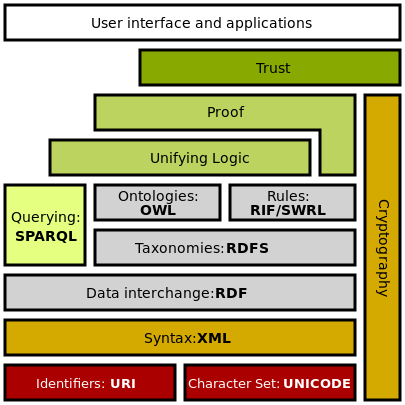
\includegraphics[scale=0.45]{pila.png}
  \caption{Struttura a strati del Web semantico}
\end{figure}

\subsection{RDF}
RDF è un semplice framework per la rappresentazione e lo scambio di metadati strutturati. Il modello concettuale che realizza RDF permette l'organizzazione delle informazioni in un insieme di triple, ognuna delle quali è composta da un soggeto, un predicato ed un oggetto. Il soggetto, ovvero la risorsa, e il predicato delle triple sono necessariamente rappresentati da un URI (Uniform Resource Identifier), mentre l'oggetto può essere un tipo di dato primitivo. Con RDF si definisce quindi un insieme di relazioni binarie che intercorrono tra due dati, ma non si forniscono regole di definizione per queste relazioni.\medskip

Un dataset RDF può essere visto e rappresentato come un digrafo, in cui i predicati sono gli archi orientati dai soggetti agli oggetti. Questa descrizione, adeguata nell'ambito della visualizzazione grafica, non è però adatta all'elaborazione automatica: si utilizza perciò una serializzazione testuale, espressa in diverse notazioni sintattiche fra cui RDF/XML, N-Triples e turtle (Terse RDF Triple Language).
Alcuni elementi che possono essere utilizzati all'interno dello stesso RDF sono termini predefiniti, classi contenitore (o collezioni) e risorse anonime (blank nodes). Inoltre è possibile utilizzare una tripla RDF come soggetto di un'altra tripla, sfruttando il meccanismo della reificazione e creando così un nuovo livello di metadati.\medskip

RDFa (RDF in attributes) è una raccomandazione W3C per l'integrazione di annotazioni semantiche all'interno dei documenti HTML e XHTML. Si possono infatti aggiungere le triple RDF sfruttando un insieme di attributi definiti dal nuovo standard, in modo tale da arricchire il contenuto informativo delle pagine Web e renderle fruibili tanto agli utenti umani quanto agli agenti che processano i metadati.
L'inserimento e la successiva estrazione di triple da un documento HTML si basa sul concetto di contesto: questo rappresenta il soggetto della tripla, al quale verranno associati tutti i valori dei successivi attributi fino al nuovo cambio di contesto.\medskip

Il primo passo verso la creazione di un linguaggio ontologico è quello di RDF-d (RDF Schema), pensato per aggiungere elementi che non possono essere espressi con il solo framework RDF. In particolare si possono definire relazioni tra termini generici invece che tra individui, con nuovi costrutti che classificano risorse e proprietà.
Tali relazioni possono ancora essere rappresentate con un grafo orientato e viene mantenuta quindi la stessa sintassi utilizzata per RDF anche per gli altri linguaggi del Web semantico (approccio same-syntax). Una dichiarazione con RDF-d può essere vista come un vincolo sulla base di dati delle triple RDF. Una importante caratteristica delle dichiarazioni in RDF/RDF-d consiste nella possibilità di parlare di dé. Si parla in questo caso di proprietà di riflessività del linguaggio.\medskip

\subsection{OWL}
Una più completa ed espressiva famiglia di linguaggi ontologici è OWL: questo strumento è stato realizzato per estendere le possibilità concesse dagli standard precedenti e costruire ontologie sempre più complesse, basate su definiti formalismi e sulle procedure di ragionamento automatico. La famiglia OWL si compone di tre differenti linguaggi: OWL-Lite, OWL-DL, OWL Full.
Questi si differenziano per le possibilità che offrono nell'ambito della potenza espressiva. La ricerca di una maggiore espressività, e quindi di una più ampia capacità di costruzione delle ontologie, sacrifica però uno degli aspetti fondamentali del Web semantico, la decidibilità logica (o la trattabilità in termini di costo computazionale nel processo di reasoning).\medskip

A differenza di quanto accade in RDF-d, OWL permette di costruire una classe enumerandone gli individui o utilizzando gli operatori insiemistici come l'unione, l'intersezione o il complemento. Inoltre è possibile costruire proprietà con vincoli come quelli di quantificazione esistenziale,  di quantificazione universale, di cardinalità minima e di cardinalità massima.\medskip

\subsection{SPARQL}
L'ultima delle tecnologie fondamentali nate per il supporto del Web semantico è SPARQL, un linguaggio di interrogazione utile per estrarre i dati codificati in basi di triple RDF. Questo strumento è stato reso standard nel 2008 dal Data Access Working Group, gruppo di lavoro del consorzio W3C. Così come SQL riflette, nella rappresentazione delle query, il modello relazionale su cui si applica, allo stesso modo SPARQL basa la propria rappresentazione sul concetto di grafo: una interrogazione viene espressa come il pattern di un grafo RDF e la risposta a tale interrogazione è costituita da tutte e sole le triple che istanziano quel pattern (graph matching).\medskip

Scendendo più in profondità nella struttura di una query SPARQL si possono idendificare diverse sezioni. Nella prima parte di dichiarano i prefissi utilizzati, si decide il tipo di risposta da ottenere (con i termini select, construct, ask e describe) e si definiscono i dataset su cui agire. A questo segue il vero e proprio graph pattern, costituito da un insieme di triple e di variabili per le quali si troveranno le corrispondenze nel dataset interrogato. Al termine si possono usare filtri e modificatori della query per ottenere un migliore controllo sulle informazioni presentate all'utente.\medskip

\section{Modello Relazionale e Modello E-R}

Il nuovo Web dei dati deve inserirsi all'interno di una ampia e complessa struttura di sistemi informativi largamente utilizzati nel mondo dell'elaborazione automatica. La manipolazione delle informazioni è comunemente affidata alla costruzione di sistemi di gestione delle basi di dati (DBMS). Nella strutturazione di una base dati si possono individuare tre fasi consecutive: la progettazione concettuale, la progettazione logica e la progettazione fisica.
La prima fase, corrispondente alla progettazione concettuale, è essenzialmente realizzata sfruttando il modello E-R, strumento principale per la rappresentazione grafica in forma di schema o diagramma. Il modello relazionale è invece il modello più diffuso per la realizzazione della progettazione logica e per le interrogazioni SQL. \MakeUppercase{è} necessario quindi sviluppare tecniche per l'integrazione di questi modelli con le nuove tecnologie del Web semantico.\medskip

Il modello relazionale si basa sul concetto matematico di relazione. Detti $D_1, D_2, ..., D_n$ una serie di $n$ domini, si definisce relazione un sottoinsieme di n-uple ordinate $(d_1, d_2, ..., d_n)$ generato dal prodotto cartesiano fra i domini $D_1 \times D_2 \times ... \times D_n$, dove $d_1 \! \in \! D_1, d_2 \! \in \! D_2, ..., d_n \! \in \! D_n$.
Nel modello relazionale, la relazione è rappresentata in forma tabellare e ogni dominio è visto come un attributo a cui è associato un nome. La mancanza di una struttura posizionale rende l'ordinamento irrilevante, ma nello stesso tempo ogni tupla deve avere elementi di tipo omogeneo rispetto agli attributi definiti.\medskip

Considerato l'esteso e trasversale uso dei modelli relazionali sono diversi i tentativi di modellazione di metadati nelle basi di dati relazionali. Esempi di tali integrazioni sono le strutture miste, in cui si associa ad ogni attributo $A$ un attributo $A_c$ per inserire le annotazioni dei valori, e le associazioni intensionali, in cui le annotazioni vengono registrate in una relazione indipendente e poi associate alle tuple corrispiondenti per mezzo della valutazione di una query.
Per lo storage e l'analisi di dati RDF è possibile creare un semplice sistema in cui, fra il DBMS e l'interfaccia utente, si inserisce un livello intermedio (middleware) in grado di tradurre le interrogazioni RDF perché il sistema relazionale sottostante possa soddisfarle. Un metodo semplice ed efficace, anche se poco efficiente, per mappare un dataset RDF in una base relazionale è quello di creare una relazione con tre attributi (soggetto, predicato ed oggetto) e costruire le tuple con le triple del dataset.\medskip

\begin{figure}[!ht]
  \centering
  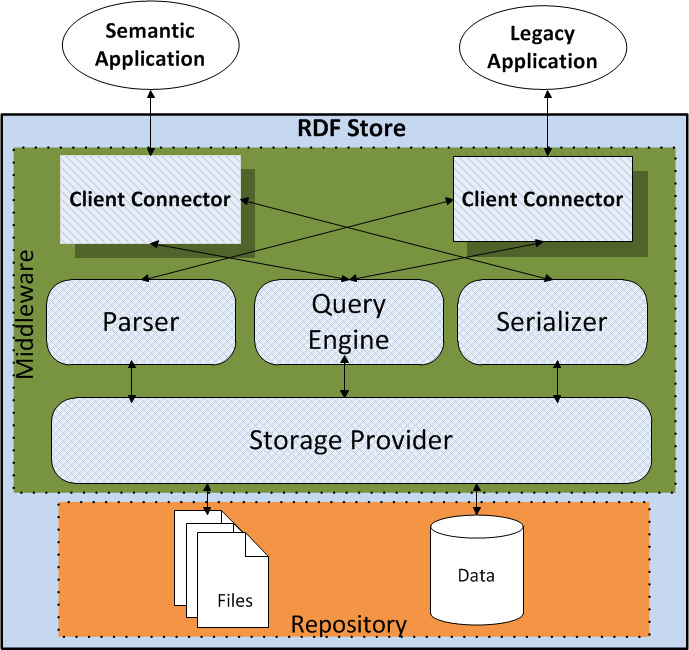
\includegraphics[scale=0.35]{rdf.jpg}
  \caption{Sistema di storage dei dati RDF}
\end{figure}

Nel modello E-R la struttura dello schema concettuale è descritta in forma grafica e definisce il livello intensionale della base di dati. I costrutti fondamentali utilizzati per tracciare i diagrammi E-R sono le entità, le relazioni, i vincoli e gli attributi. Le entità rappresentano le classi degli oggetti di interesse mentre le relazioni sono associazioni che legano due o più entità. Una base di dati, così come una ontologia, è un metodo per rappresentare un insieme di informazioni: sembra quindi immediata, almeno dal punto di vista speculativo, la traduzione della struttura definita da uno schema E-R in un dominio ontologico che sia fedele alle regole imposte dal Web semantico. Questa operazione è in effetti possibile, sebbene esistano delle limitazioni e sia necessario tenere in considerazione le numerose differenze che intercorrono fra un diagramma e un linguaggio come OWL.\medskip

La prima divergenza che può essere notata è l'ipotesi di mondo chiuso, assunzione secondo la quale una dichiarazione è vera se e solo se è effettivamente definita ed è considerata falsa se il suo valore di verità non è noto. Questa ipotesi caratterizza generalmente i modelli relazionali. Al contrario, OWL opera l'assunzione opposta, l'ipotesi di mondo aperto, in cui è ammessa una conoscenza incompleta dei dati di interesse. La stessa divergenza si trova sull'ipotesi di unicità del nome: l'idea per cui due nomi diversi si riferiscano ad entità diverse non è accettata a priori in OWL.\medskip

Dal punto di vista dei costrutti, le entità di un diagramma E-R possono essere direttamente tradotte nelle classi OWL, mantenendo la struttura tassonomica con l'uso di superclassi e sottoclassi. Diversi generi di vincoli devono essere aggiunti per determinare le restrizioni sugli individui che possono appartenere ad una classe. \MakeUppercase{è} importante notare che, alla pari dello schema E-R, le sottoclassi ereditano le proprietà delle rispettive superclassi.
Le relazioni binarie fra entità del diagramma sono tradotte nelle Object Properties, proprietà che legano individui di due classi (non necessariamente distinte), mentre gli attributi delle entità si traducono in Datatype Properties, che legano un individuo a un tipo di dato primitivo (integer, float, string...). In OWL è possibile definire il dominio ed il range delle proprietà ed aggiungere un set di restrizioni di quantità e cardinalità per gli individui che sono coinvolti dalle proprietà stesse. Non è possibile al contrario modellizzare fedelmente gli attributi delle relazioni e soprattutto definire le chiavi primarie di una classe, presenti e fondamentali nel modello relazionale.\medskip

\chapter{Vector Space Model}
\section{Sistemi di Raccomandazione}

I sistemi di raccomandazione sono software di manipolazione del contenuto informativo, largamente utilizzati per gestire grandi quantità di dati e selezionare gli stessi in funzione di una migliore fruizione da parte degli utenti a cui sono rivolti. Questi sistemi vengono impiegati in modo evidente soprattutto dalle piattaforme online che operano in ambito e-commerce, come Amazon, e streaming on demand, fra cui Netflix e Spotify. Un sistema di raccomandazione si rende perciò indispensabile in tutte le occasioni in cui è necessario contenere il volume delle informazioni e creare un metodo di filtraggio per la visualizzazione e la presentazione. L'obiettivo: aiutare le persone ad effettuare scelte in base alle proprie preferenze. In modo più formale: detto $C$ l'insieme degli utenti e $D$ l'insieme degli elementi, il migliore elemento per un utente è quello che massimizza la funzione di utilità $u(c,d)$.

\[
\forall \, c \in C, \quad \hat{d}_c = \argmax_{d \in D} \, u(c, d)
\]

\medskip

La prima fase di cui si compone un sistema di raccomandazione è la raccolta dei dati relativi agli oggetti di interesse per l'applicazione e alla profilazione degli utenti che ne usufruiscono. Il sistema migliorerà il servizio offerto solo nel momento dispone di sufficiente conoscenza: questa fase è quindi di fondamentale importanza per il conseguimento di buoni risultati, indipendentemente dalla tecnica di filtraggio messa in atto. Per quanto detto emerge in modo chiaro la stretta relazione che intercorre fra i sistemi di raccomandazione e l'attuale ambito definito Big Data Analysis.
Gli input su cui lavorerà il sistema possono essere forniti esplicitamente (ad esempio, attraverso un metodo di rating) o, in modo più sofisticato, ottenuti mediante l'osservazione del comportamento degli utenti ed una successiva deduzione delle loro preferenze. Quest'ultimo metodo resta, allo stato dell'arte, meno performante del precedente, anche se rappresenta al meglio l'idea sottostante un sistema di raccomandazione ed è immune dal problema del bias.\medskip

In base alla tecnica usata per ottenere le raccomandazioni, i sistemi possono essere classificati in quattro categorie: filtraggio content-based, filtraggio collaborativo, filtraggio ibrido e filtraggio semantic-social. Le tecniche content-based sfruttano gli attributi degli oggetti di interesse per ottenere i risultati piuttosto che le informazioni sugli utenti.
Questo criterio è principalmente utilizzato nell'analisi di documenti testuali e pagine web ed estende alcuni degli approcci tipici dell'information retrieval. Si impiegano a tal proposito metodi quali Vector Space Model e Neural Networks per estrarre relazioni fra i documenti e fornire le raccomandazioni agli utenti. Il principale svantaggio risiede nella necessità di una conoscenza approfondita delle feature (caratteristiche) sulle quali fondare la valutazione. Nello stesso tempo però non si richiede la profilazione degli utenti e la condivisione delle loro informazioni, favorendo così la protezione della privacy.\medskip

Il metodo collaborativo crea dei suggerimenti utilizzando la similarità tra gli utenti. Si registrano le scelte del maggior numero di persone e si forniscono raccomandazioni associandole in gruppi definiti neighborhood. Utenti con stesse preferenze possono quindi scambiare indirettamente diverse informazioni fra loro, suggerendo nuovi contenuti attraverso il sistema.
In questo caso, l'utilità $u(c,d)$ dell'elemento $d$ per la persona $c$ è basata sull'utilità $u(c',d)$ assegnata a $d$ dalle persone $c' \in C' \subseteq C$ che sono simili a $c$. Anche questo metodo, nonostante sia più dinamico e attuale, non è esente da particolari svantaggi, primi fra tutti la scalabilità, la sparsità dei dati e la mancanza di sufficienti informazioni sugli utenti che si autenticano per la prima volta o che non condividono il loro profilo.\medskip

Le tecniche usate per la realizzazione dell'approccio collaborativo sono svariate e spesso mutuate dai settori del machine learning e del data mining (model-based collaborative filtering). Si parla quindi di modelli probabilistici e algoritmi di apprendimento come le reti neurali, ma anche regole di associazione, alberi di decisione e clustering.
In questi algoritmi, come per la funzione utilità, il rating $r_{c,d}$ della persona $c$ per l'oggetto $d$ viene calcolato sulla base dei rating $r_{c',d}$ delle persone più simili a $c$. In particolare è possibile usare una media pesata dei rating rispetto a tutti gli utenti $c'$ del tipo

\[
r_{c,d} = \widetilde{r}_c + k \sum_{c' \in C'} sim(c,c') \cdot (r_{c',d} - \widetilde{r}_{c'})
\]

dove

\begin{itemize}
  \item $k$ è un fattore normalizzante del tipo $k = 1 / \sum |sim(c,c')|$
  \item $\widetilde{r}_c$ è il rating medio di una persona, $\widetilde{r}_c = (1/|D_c|) \sum_{d \in D_c} r_{c,d}$
  \item $D_c$ è l'insieme degli elementi relativi a $c$, ovvero $D_c = \{d \in D \, | \, r_{c,d} \neq 0\}$
  \item $sim(c,c')$ è la similarità fra $c$ e $c'$
\end{itemize}

\medskip

Nel tentativo di superare le criticità ad ottenere il miglior sistema di raccomandazione è stato sviluppato l'approccio ibrido, che integra i metodi descritti in precedenza e li sintetizza con strategie differenti. Infine, negli ultimi anni, sono nati nuovi sistemi ispirati al crescente utilizzo dei social network.
L'approccio semantic-social si fonda perciò sulla modellazione delle reti sociali e delle interazioni fra persone ed oggetti. Le reti sono rappresentate da strutture astratte come i grafi e possono essere visitate con i tradizionali algoritmi di ricerca su grafo come depth-first search (DFS).\medskip

\section{TF-IDF e Cosine Similarity}

Come descritto in precedenza, uno dei metodi utilizzati per la realizzazione di un sistema di raccomandazione content-based è il Vector Space Model. Questo modello,  adoperato spesso nell'ambito dell'information retrieval, consiste essenzialmente nel rappresentare gli elementi che dovranno essere raccomandati agli utenti in uno spazio vettoriale n-dimensionale.
Ogni elemento $d \in D$ sarà descritto da un vettore del tipo $d_j = (w_{1j}, w_{2j}, ..., w_{nj})$. La dimensione dei vettori dipende dal numero di caratteristiche sulle quali si vuole basare il sistema, ad esempio un insieme di parole chiave nel caso in cui, come spesso accede, gli elementi rappresentano dei documenti testuali.\medskip

Per quanto detto, è necessario stabilire il modo in cui calcolare le componenti $w_{ij}$ dei vettori. Il primo e più immediato procedimento consiste nell'assegnare solo coefficienti di tipo binario in base alla presenza di una determinata caratteristica nell'elemento analizzato. Un modello così semplice è però insufficiente per ottenere buoni risultati. Si estende perciò questo metodo contando il numero di occorrenze delle feature ricercate.
\MakeUppercase{è} possibile per esempio contare le occorrenze dei termini rilevanti all'interno di un documento. Alcune parole molto frequenti possono però essere poco rilevanti e portare a classificazioni poco precise. Si ricorre quindi ad un modello più complesso, definito TF-IDF (term frequency - inverse document frequency). Il primo passo è calcolare la frequenza dei termini con elementi di normalizzazione. Detto $count(t,d)$ il numero di occorrenze del termine $t$ nel documento $d \in D$, è possibile utilizzare una delle seguenti formule
\begin{gather*}
  t\!f(t,d) = \frac{count(t,d)}{|d|} \\
  t\!f(t,d) = 1 + \log_{10}(count(t,d)) \\
  t\!f(t,d) = k + (1-k) \frac{count(t,d)}{max\{count(t',d) : t' \in d\}}
\end{gather*}
A questa misura si aggiunge un termine correttivo, detto inverse document frequency, utile per tenere in considerazione la rilevanza di una parola rispetto alle sue occorrenze nella totalità dello spazio dei documenti. Questo valore sarà più grande se il termine appare più raramente
\[
idf(t) = \log \frac{|D|}{|\{d \in D : t \in d\}|}
\]
Il calcolo della componente relativa a $t$ nel vettore sarà quindi dato dalla combinazione dei valori precedentemente calcolati, ovvero
\[
w_{ij} = t\!fidf_{i,j} = t\!f(i,j) \cdot idf(i)
\]

\medskip

Una volta ricavati tutti i coefficienti dei vettori che rappresentano gli elementi del sistema, la raccomandazione può essere effettuata in base alla distanza di questi vettori. Più vicini sono i vettori, più simili saranno gli elementi sottostanti. In altre parole quindi si calcola, per ogni elemento, l'insieme dei suoi correlati: un utente potrà infatti apprezzare questi ultimi se ha scelto in precedenza l'oggetto di riferimento. Per ottenere la distanza fra due vettori è possibile certamente utilizzare la tradizionale distanza euclidea. Più utilizzata e più robusta per alcune situazioni inconsuete è invece la tecnica del coseno di similitudine: dati i vettori $d_1$ e $d_2$ si calcola il coseno dell'angolo fra loro compreso
\[
\cos(d_1, d_2) = \frac{d_1 \cdot d_2}{||d_1|| \, ||d_2||} = \frac{d_1^T d_2}{||d_1|| \, ||d_2||} = \frac{\sum_{i} w_{i1} w_{i2}}{\sqrt{\sum_{i} w_{i1}^2} \sqrt{\sum_{i} w_{i2}^2}}
\]

\begin{figure}[!ht]
  \centering
  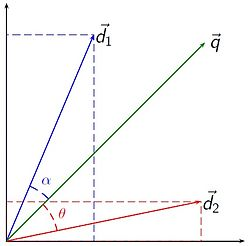
\includegraphics[scale=0.9]{vsm.jpg}
  \caption{Distanza fra vettori}
\end{figure}

Il risultato ottenuto avrà sempre un valore compreso tra $0$ e $1$, se le componenti dei vettori impiegati sono numeri razionali non negativi. Un risultato pari ad uno corrisponde ad una maggiore somiglianza degli elementi considerati. Il coseno di similitudine non fa altro che dividere il prodotto scalare fra i vettori con la loro norma, in modo tale che documenti possano avere valori maggiori in base alla loro lunghezza. In sostituzione di questa tecnica, altre misure utilizzate sono il coefficiente di Dice
\[
sim(d_1, d_2) = 2 \, \frac{d_1 \cdot d_2}{||d_1||^2 + ||d_2||^2} = 2 \, \frac{\sum_{i} w_{i1} w_{i2}}{\sum_{i} w_{i1}^2 + \sum_{i} w_{i2}^2}
\]
e il coefficiente di Jaccard
\[
sim(d_1, d_2) = \frac{d_1 \cdot d_2}{||d_1||^2 + ||d_2||^2 - d_1 \cdot d_2} = \frac{\sum_{i} w_{i1} w_{i2}}{\sum_{i} w_{i1}^2 + \sum_{i} w_{i2}^2 - \sum_{i} w_{i1} w_{i2}}
\]

\medskip

Nonostante il vasto impiego dei modelli probabilistici, il Vector Space Model mantiene un posto di rilievo ed interesse nello studio dei sistemi di raccomandazione. Diversi sono i tentativi di integrare questo metodo con l'approccio collaborativo e di estenderlo per il superamento di alcuni limiti, quali la necessaria indipendenza interna dei termini del documento analizzato, la perdita dell'ordinamento e la mancata considerazione del contesto semantico. Inoltre ha il vantaggio di essere un metodo di semplice implementazione, basato esclusivamente sull'algebra lineare ed efficace nel caso di insieme di dati poco complessi.

\chapter{Architettura}

\section{Struttura}

Il progetto si compone di diverse fasi, ognuna delle quali costituita da un modulo software autoconclusivo e sviluppata con linguaggi e framework differenti.\medskip

In una fase preliminare viene disegnato il diagramma E-R sulla base dei dataset relativi al dominio di interesse. Questo costituisce il modello dei dati su cui viene creata l'ontologia OWL per modellizzare le entità e le relazioni del dominio: a tale scopo è stato impiegato l'editor Protégé, ampiamente utilizzato nell'ambito dello sviluppo delle basi di conoscenza.
L'ontologia così formata viene successivamente popolata dai dati forniti da alcuni dei dataset della piattaforma Kaggle, opportunamente ristrutturati sottoforma di insieme di triple per rispondere ai requisiti di RDF. Il risultato di questa elaborazione consiste in un documento testuale in formato RDF/XML. Il lunguaggio usato in questa fase è Python, con la libreria esterna RDFLib.\medskip

La seconda fase si pone come obiettivo quello di individuare le relazioni che intercorrono fra i dati analizzati ovvero di trovare, per ogni individuo presente nell'ontologia, un insieme di elementi ad esso correlati. A questo riguardo si è ricorso alla tecnica di raccomandazione del Vector Space Model, utile per fornire all'utente indicazioni relative alla similarità tra gli oggetti. Il prodotto di questa attività consiste in un nuovo documento del tutto analogo al precedente ma arricchito con le nuove informazioni estratte. Java ed il framework Jena sono gli strumenti adoperati per l'implementazione del metodo descritto.\medskip

La terza ed ultima fase è preposta alla presentazione dei dati elaborati in precedenza. La visualizzazione avviene, utilizzando uno dei browser disponibili, nella tradizionale forma tabellare e fornisce funzioni supplementari per la navigazione delle informazioni. Queste ultime vengono reperite attraverso l'esecuzione di opportune query SPARQL dal documento prodotto nel corso delle prime due fasi. Lo sviluppo è stato realizzato con metodologia server-side impiegando in particolar modo Node.js ed il framework Express.js.

\section{Strumenti}
\subsection{Protégé}

Protégé-OWL è un editor visuale pensato per la creazione, la modifica e l'esportazione delle ontologie per il Web semantico. Nato come progetto per modellare il dominio biomedico presso l'università di Stanford, attualmente è lo strumento più noto per la gestione delle ontologie OWL, grazie anche ai numerosi plug-in di cui dispone e alla semplicità di utilizzo. Protégé consente quindi la creazione di un insieme di classi, di oggetti che afferiscono a queste classi e di proprietà che le mettono in relazione tra loro. A questo si aggiungono le annotazioni, l'importazione dei file esterni per la modularità e i prefissi che vengono usati nell'ontologia.\medskip

Le classi sono organizzate in una gerarchia (asserted hierarchy) nella quale la superclasse predefinita è {\it owl:Thing}. Queste andranno a rappresentare le entità da modellare nel dominio. Le classi possono essere dichiarate equivalenti o disgiunte da altre classi, e si servono dei vincoli di restrizione per limitare gli individui che possono essere istanziati. Del tutto analogo è il procedimento per la creazione delle proprietà, divise in Object Properties e Data Properties, per le quali è possibile definire le entità che compongono il dominio ed il range.

\subsection{Jena}

Jena è un framework open source per lo sviluppo in Java di applicazioni legate all'ambito del Web semantico. In particolare, la struttura delle API (Application Programming Interface) è progettata per la gestione di dati RDF: vengono infatti fornite diverse funzioni volte alla creazione, alla serializzazione e al parsing dei documenti strutturati in triple. \MakeUppercase{è} possibile creare nodi tipati e containers, ma anche definire classi wrapper per la manipolazione di vocabolari implementati contestualmente o predefiniti (come il celebre Dublin Core).\medskip

Per accedere ai dati memorizzati in un modello RDF, sia esse contenuto in memoria principale o meno, Jena espone delle API per l'esecuzione di una query SPARQL e la successiva visita iterativa dei risultati ottenuti. Le classi QueryFactory, QueryExecution e ResultSet consentono il conseguimento di questo obiettivo. \MakeUppercase{è} consentito infine eseguire le stesse operazioni interrogando i dati RDF in remoto per mezzo dei corrispondenti endpoint.

\subsection{Node.js}

Node.js è un ambiente run-time per l'esecuzione di codice JavaScript lato server e la produzione di pagine web dinamiche. Consente

\chapter{Implementazione}
\section{I dati}

Nello sviluppo del presente progetto sono stati utilizzati diversi dataset che coinvolgono dettagliate informazioni relative all'ambito della multimedialità. Tali dataset sono stati ricavati dal vasto archivio presente sulla piattaforma online Kaggle e afferiscono a quattro principali categorie: libri, film, album musicali e videogiochi. I dati così ottenuti, contenuti in altrettanti file csv, sono il punto di partenza per l'intero sviluppo successivo del software.\medskip

Dopo un iniziale preprocessamento dei file, utile per verificare la consistenza ed eliminare eventuali informazioni errate rispetto al dominio in esame, è possibile procedere con le prime fasi che caratterizzano il workflow. \MakeUppercase{è} stato perciò realizzato il diagramma E-R per definire in forma grafica lo schema concettuale dei dati presi in considerazione. Questo diagramma non si rende strettamente necessario per la successiva creazione dell'ontologia, ma si utilizza a tale scopo in questo progetto per mostrare come possa essere effettuata la traduzione fra i due modelli e come possano essere integrate le tecnologie del Web semantico con il più tradizionale metodo di progettazione delle basi di dati.\medskip

\begin{center}
\scalebox{.87}{
\begin{tikzpicture}[node distance=0.5cm, every edge/.style={link}]
  \node[entity] (media) {Media};
  \node[isa] (isa) [below=0.5cm of media] {IS-A} edge (media);
  \node[entity] (album) [below=0.5cm of isa] {Album} edge (isa);
  \node[attribute] (genre) [left=1.0cm of album] {Genre} edge (album);
  \node[attribute] (title) [above left=1.0cm of album] {\key{Title}} edge (album);
  \node[attribute] (year) [below left=1.0cm of album] {Year} edge (album);
  \node[attribute] (rating) [below=1.0cm of album] {Rating} edge (album);
  \node[relationship] (rec) [right=0.5cm of album] {RecBy};
  \node[relationship] (lab) [below right=1.5cm of album] {LabBy};
  \node[entity] (artist) [right=0.5cm of rec] {Artist};
  \node[entity] (label) [right=3.0cm of lab] {Label};
  \draw[link] (album) edge (rec) (rec) edge (artist);
  \draw[link] (album.-25) edge (lab) (lab) edge (label);
  \node[isa] (isa2) [above=0.25cm of artist] {IS-A} edge (artist);
  \node[isa] (isa3) [above=0.25cm of label] {IS-A} edge (label);
  \node[entity] (org) [above=0.5cm of isa3] {Organization} edge (isa3);
  \node[isa] (isa4) [above=0.35cm of org] {IS-A} edge (org);
  \node[entity] (person) [above=0.45cm of isa2] {Person} edge (isa2) edge (isa4);
  \node[entity] (agent) [above=0.5cm of isa4] {Agent} edge (isa4);
\end{tikzpicture}
}
\end{center}

Nello schema descritto, e allo stesso modo nei pragrafi successivi, si riduce lo studio all'ambito degli album musicali per una maggiore chiarezza espositiva. Il numero di classi e relazioni prese in considerazione quindi è molto maggiore rispetto a quanto viene rappresentato. Le altre categorie trattane nel software sono sviluppate in modo del tutto analogo.

\section{L'ontologia}

Parte del processo di sviluppo del progetto coinvolge certamente la creazione e l'interrogazione delle ontologie OWL. Questa fase coinvolge quindi la traduzione del diagramma E-R descritto in una base ontologica, sfruttando gli strumenti messi a disposizione dalla piattaforma Protégé-OWL. Come detto in precedenza, la traduzione non può avvenire senza tenere conto delle fondamentali differenze che intercorrono fra i due modelli di dati.\medskip

L'entità Album, come le altre coinvolte nel dominio analizzato, diviene una classe dell'ontologia. Viene così creata una tassonomia che struttura gerarchicamente tutte le entità coinvolte, secondo le relazioni is-a mostrate. Inoltre si rende necessario esplicitare in OWL la disgiunzione fra le classi che hanno fra loro intersezione vuota, ovvero i cui individui non possono essere nello stesso momento oggetti di classi diverse. Album viene dichiarata quindi sottoclasse di Media e disgiunta da Book, Movie e Game. Gli attributi Title, Genre, Year e Rating divengono le Data Properties della classe e sono dichiarati functional in base alla loro cardinalità, mentre le relazioni RecordedBy e LabeledBy sono modellate nelle Object Properties, che legano una classe ad un'altra. Queste ultime possono essere descritte attraverso numerose caratteristiche, quali ad esempio functional, transitive, symmetric e reflexive. \MakeUppercase{è} importante notare come nell'ontologia viene perso il concetto di chiave primaria: l'attributo Title, come tutte le Data Properties, non può essere definito Inverse functional e questo impedisce la possibilità di considerarlo come una chiave senza fare riferimento al modello E-R originario. Al termine di questa fase, la base di conoscenza formata viene esportata in un documento OWL in formato RDF/XML*.\medskip

Il documento così generato viene popolato in un secondo momento con un insieme di triple che codificano le informazioni dei dataset utilizzati. Con il supporto di Python vengono quindi letti i documenti csv e, una volta raggruppati in triple del tipo soggetto-predicato-oggetto, sono aggiunti i dati all'ontologia. Questo processo è agevolato dalla libreria RDFLib, che mette a disposizione diverse funzioni per istanziare un grafo RDF e manipolare le sue componenti: è possibile infatti accrescere il contenuto interno del grafo, ma anche eseguire il parsing di un documento e la serializzazione dei contenuti per la conseguente scrittura su file. Al termine di questa fase si otterrà come risultato un documento completo e arricchito di tutte le informazioni necessarie, che rispetta nella struttura alcuni dei principi descritti nell'ambito del Web semantico. Sarà definito quindi non solo il livello intensionale, ma anche il livello estensionale della base di conoscenza, composta ora dalle definizioni di classi e proprietà e da tutti gli individui aggiunti con il semplice ma utile codice scritto. Nessuna libreria aggiuntiva è richiesta per l'esecuzione del programma.

\section{La correlazione}

Nello studio e nell'analisi di grandi quantità di dati è fondamentale cercare di estrarre le relazioni nascoste che intercorrono fra le informazioni, i pattern sottesi, i collegamenti implicitamente creati. A questo scopo è possibile scrivere opportuni moduli software per l'osservazione delle suddette relazioni. Nel presente progetto sono state utilizzate le tecniche del Vector Space Model per ottenere le correlazioni degli oggetti presenti nell'ontologia.\medskip

Per il conseguimento dell'obiettivo dichiarato si è optato quindi per un metodo di filtraggio content-based: questo presenta infatti numerosi vantaggi se correttamente immerso nel contesto sviluppato. Il primo aspetto è sicuramente quello di mantenere in un ruolo di assoluta centralità l'informazione e la sua interpretazione da parte degli elaboratori. A questo si aggiunge una sorprendente efficacia, ottenuta a dispetto della semplicità del modello algebrico impiegato. I risultati inoltre non necessitano di alcuna azione da parte degli utenti e possono essere quindi ricavati anche in assenza di meccanismi di autenticazione e memorizzazione delle preferenze.\medskip

Il sistema di raccomandazione sviluppato, in grado di suggerire per ogni elemento i suoi correlati, è stato realizzato con Java ed il relativo framework Jena. Quet'ultimo consente l'uso di classi e di metodi per istanziare un modello, per estrarne i dati attraverso l'uso di appropriate interrogazioni ed per la finale scrittura dei dati. Al termine dell'esecuzione viene corredata l'ontologia con le informazioni ricavate. A questo proposito si aggiunge una nuova Object Property che mette in relazione un individuo di una classe con un altro individuo della stessa classe. Questa proprietà viene definita correlatedWith e restituisce l'idea di affinità fra i due oggetti coinvolti.\medskip

Le prime classi Java scritte in questa fase sono le classi in grado di istanziare gli elementi del dominio e prendono il nome dalle quattro categorie da cui provengono questi stessi elementi, ovvero Album, Book, Movie e Game. La classe MyQuery contiene invece i metodi responsabili per la corretta esecuzione delle interrogazioni SPARQL e della successiva organizzazione delle risposte ottenute in adeguate strutture dati. Questi metodi servono per estrarre dal documento OWL tutte e sole le triple che afferiscono ad una determinata categoria, ad esempio quella degli Album, ed effettuare controlli sull'integrità dei contenuti così ricavati.\medskip

Le operazioni che implementano il vero e proprio metodo del Vector Space Model sono infine contenute nelle classi TFIDF, Similarity e Recommender. Le prime due, come suggerisce il nome stesso, sono preposte rispettivamente alla creazione dei vettori che rappresenteranno gli individui con il calcolo delle loro componenti e alla misura della distanza fra i suddetti vettori attraverso la misura del coseno di similitudine. In particolare, il numero delle componenti dei vettori  stabilito in base alle caratteristiche considerate come rilevanti ai fini della correlazione. Ogni album musicale ad esempio viene descritto con un vettore di tre componenti, ognuna delle quali relativa all'artista che lo ha prodotto, all'anno in cui è uscito e ai generi musicali a cui appartiene. Questi sono gli aspetti che in fase di progettazione sono stati individuati per stabilire le correlazioni. I vettori fra loro più vicini, ovvero con un angolo compreso di minore ampiezza, sono considerati in relazione fra loro e possono essere suggeriti come simili ad un utente fruitore del serizio. La classe Recommender non fa altro che chiamare i metodi delle due precedenti per rendere effettivo il sistema di raccomandazione. Un ultimo file, contenente la classe Main, è responsabile della ripetizione del processo per ogni contenuto estratto dall'interrogazione e della scrittura dei correlati all'interno del documento che contiene l'ontologia e l'insieme di triple, attraverso l'opportuna proprietà in precedenza definita.

\section{La visualizzazione}



\section{La paginazione e la ricerca}




\chapter{Conclusioni}
\section{Risultati}
%Questo documento sarà del tipo seguente

%\lstset{language=XML}
%\insertcode{myontology.owl}

\chapter*{Argomenti}
\begin{enumerate}
  \item Correlazione (Java e Jena)
  \item Query semantiche (da SQL a SPARQL)
  \item Rappresentazione Web (UI)
  \item Node.js e Express.js
  \item Paginazione e ricerca (JQuery)
  \item Confronto prestazioni
  \item Reverse Engineering e ottimizzazione delle prestazioni
  \item Risultati ottenuti
\end{enumerate}

\backmatter
\cleardoublepage
%\addcontentsline{toc}{chapter}{\bibname}
%\phantomsection
%\bibliographystyle{sapthesis} % BibTeX style
%\bibliography{bibliography} % BibTeX database without .bib extension

\end{document}
